
% Diese Grundkonfiguration wurde von der Beispielkonfiguration übernommen
\documentclass[12pt,pdftex,parskip=half]{scrartcl}
\usepackage[ngerman]{babel}
\usepackage[utf8]{inputenc}  \usepackage[T1]{fontenc}
\usepackage{graphicx}
\usepackage{xcolor}
\usepackage{pdfpages}
\usepackage{url}


% ändert die Schriftart im gesamten Dokument (nur eine Zeile darf aktiv sein) (Auswahl: http://www.tug.dk/FontCatalogue/)
\usepackage{dejavu}

% hiermit kann das €-Zeichen direkt eingegeben werden
\usepackage{eurosym}  \DeclareUnicodeCharacter{20AC}{\euro}

% Informationen, die in der pdf-Datei stehen
\usepackage[pdftitle={}, pdfauthor={}, pdfstartview=FitH, colorlinks=true, linkcolor=black, urlcolor=blue, citecolor=black]{hyperref}

% Seitenränder
\usepackage{geometry}
\geometry{a4paper,left=20mm,right=20mm,bottom=20mm,top=15mm,bindingoffset=0mm,includehead,includefoot}

% Kopf- und Fußzeile jeweils mit Linie
\usepackage{fancyhdr} \pagestyle{fancy} \renewcommand{\headwidth}{\textwidth}
\renewcommand{\headrulewidth}{0.4pt} \lhead{} \chead{} \rhead{}
\renewcommand{\footrulewidth}{0.4pt} \lfoot{} \cfoot{\small \today} \rfoot{\small \thepage}

% kein Erstzeileneinzug und etwas mehr Zeilenabstand
\setlength{\parindent}{0pt}  \linespread{1.1}

% Angaben für das Literaturverzeichnis
\usepackage[backend=bibtex, style=alphabetic, bibencoding=ascii]{biblatex}
\addbibresource{vorlage.bib}
\usepackage{csquotes}

% Einstellungen für HTML-Sourcecode
\usepackage{listings}
\lstset{language=HTML,
    frame=single,
    basicstyle=\footnotesize\ttfamily,
    breaklines=true,
    breakatwhitespace=true,
    classoffset=1,
    commentstyle=\slshape\color{cyan},
    framextopmargin=2pt,
    framexbottommargin=2pt,
    identifierstyle=\color{orange},
    keywordstyle=\color{red},
    morekeywords={main,cin,cout}, keywordstyle=\bfseries\color{magenta},
    rulecolor=\color{black!40},
    showspaces=false, showstringspaces=false,
    stringstyle=\color{blue},
    tabsize=2,
    title=\lstname
}


% Beginn des Textes
\begin{document}


% Deckblatt
\begin{titlepage}
    \begin{center}
        \vfill {{\Large Bestellverwaltung GUI für Nordwind Datenbank}}
        \vfill {Lernfeld 6: Entwickeln und Bereitstellen von Anwendungssystemen\\Herr Goebel}
        \vfill {von\\Yannick Lapp\\\today} %todo: Datum anpassen auf Abgabedatum
    \end{center}
\end{titlepage}


% Inhaltsverzeichnis
\tableofcontents
\clearpage


% 1. Aufgabenstellung
\section{Aufgabenstellung}

Es sollte eine Bestellverwaltung für die Nordwind Datenbank erstellt werden.
Die Anwender sollen die Bestellverwaltung über eine Webseite nutzen können.

Die Nordwind Datenbank ist eine Datenbank, die ursprünglich mit Microsoft Office als Demodatenbank mitgeliefert wurde. Mittlerweile ist sie aber weiträumig für Lern- und Übungszwecke in Gebrauch und ist für die meisten Datenbankmanagementsysteme verfügbar.\\
Zum Testen dieses Projekts wurde eine
\href{https://www.apachefriends.org/de/index.html}{xampp}
Installation mit bereits integrierter Nordwind Datenbank verwendet, es kann aber durch Anpassen der Datenbankverbindungsparameter mit einem beliebigen MySQL Datenbankserver genutzt werden.

Auf der nächsten Seite befinden sich die genauen Aufgabenstellungen.

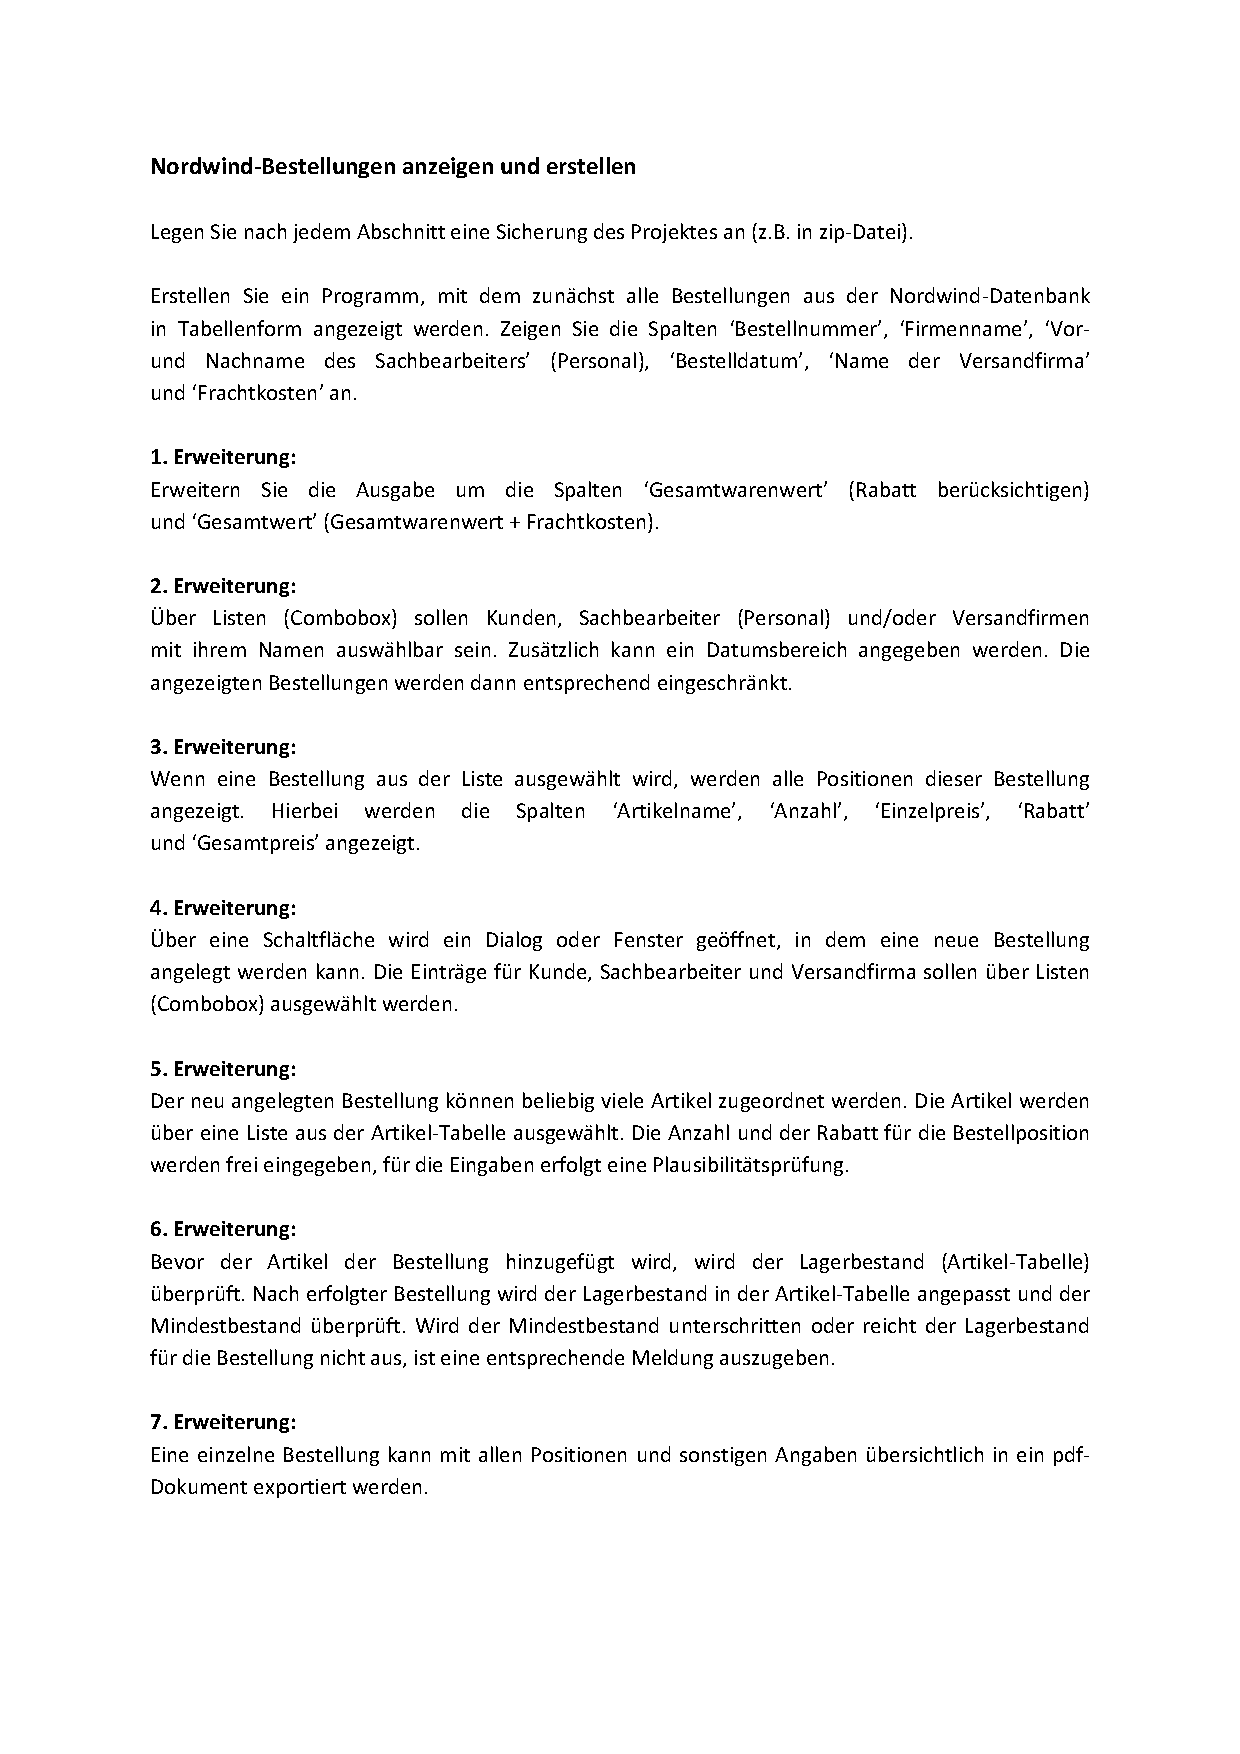
\includepdf[pages=1,scale=0.9,frame=true]{PDFs/Nordwind-BestellungenAufgaben}


% 2. Grober Überblick
\section{Überblick der umgesetzten Anwendung}


    % 2.1
    \subsection{Quellcode}

    Der Quellcode für die Anwendung kann in diesem git repository eingesehen werden:\\
    \href{https://github.com/ylapp1/Northwind-WebOrder}{https://github.com/ylapp1/Northwind-WebOrder}

    Git ist ein Versionskontrollsystem, damit kann man den Verlauf der Erstellung der Anwendung nachverfolgen, zu früheren Versionen zurückspringen und die aktuellen Änderungen im Vergleich zur neusten Version in seinem lokalen Klon betrachten.

    Im Repository kann auch der Commit Verlauf verfolgt werden, das heißt welche Dateien wann geändert wurden und zu welchem "`Änderungsblock"' sie gehören.\\
    Das sollten normalerweise z.B. das Hinzufügen von neuen Funktionen sein, in diesem Falle wären zum Beispiel die Erweiterungen gute Commits gewesen.\\
    Das wurde hier bis Erweiterung 4 auch so umgesetzt, danach wurde aber das bisherige selbst gebaute Tabellen-Element ersetzt durch bootstrap-table und die jQuery-UI-Dialoge wurden ersetzt durch bootstrap Dialoge, damit die Seite einen einheitlichen Stil hat.\\
    Damit kamen sehr viele Änderungen auf einmal in einem commit und die darauf folgenden commits zielten nur noch darauf ab, die Anwendung mit den Änderungen aus dem großen commit wieder zum Laufen zu bekommen.\\
    Das ist aber kein Problem, da der branch sowieso nur ein feature branch ist, d.h. er wird in den Hauptbranch (hier "`master"') gesquasht (= zu einem einzigen Commit zusammengefasst und an den Hauptbranch angehängt).


    Der Quellcode ist in Englisch geschrieben.
    Die Sprache der GUI ist aber hardgecoded Deutsch.\\
    Im Code befinden sich auch Kommentare auf Englisch, die Funktionen, Klassen und manche Code Schnipsel näher beschreiben.\\
    Dieses Dokument soll nur einen relativ groben Überblick über die Funktionsweise der Anwendung und der einzelnen Klassen geben.
    Einen tieferen Einblick kann der Quelltext und die sich darin befindenden Kommentare liefern.



    \newpage


    % 2.2 Screenshots
    \subsection{Beispiel Screenshots}

        \begin{figure}[!htb]
            \centering
            \frame{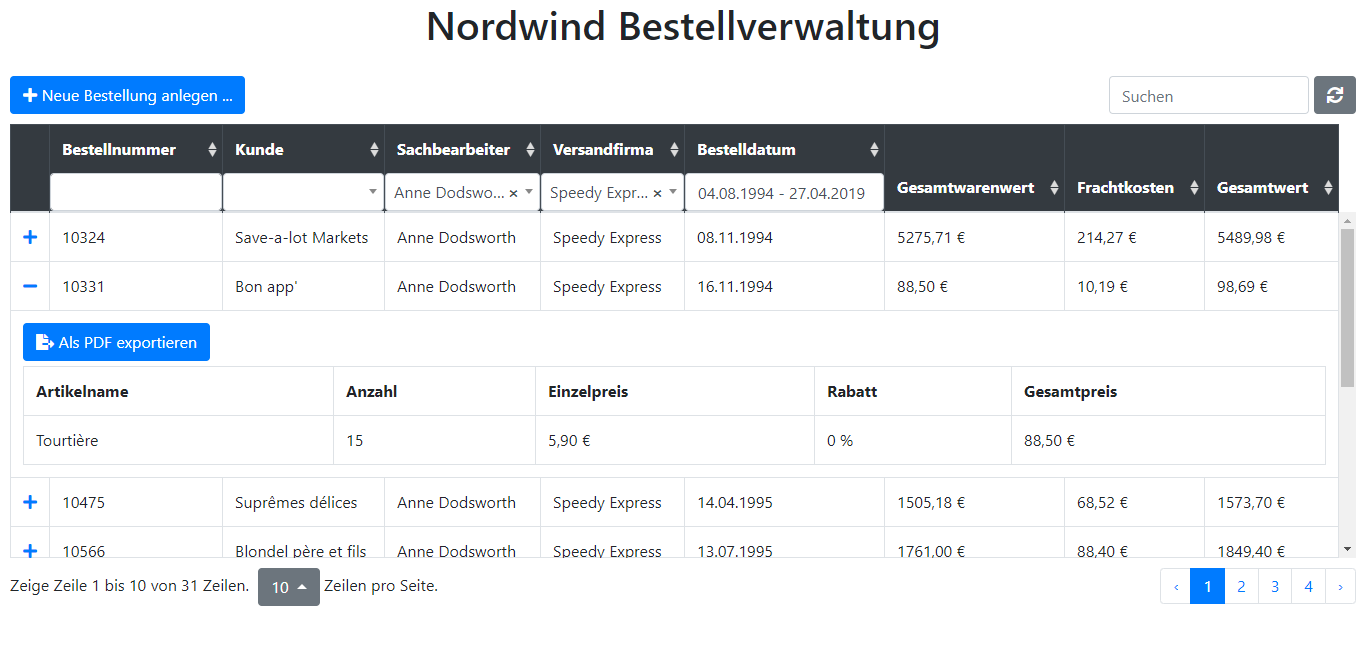
\includegraphics[scale=0.45]{Screenshots/OrdersTable.png}}
            \caption{Hauptseite}
        \end{figure}

        \begin{figure}[!htb]
            \centering
            \frame{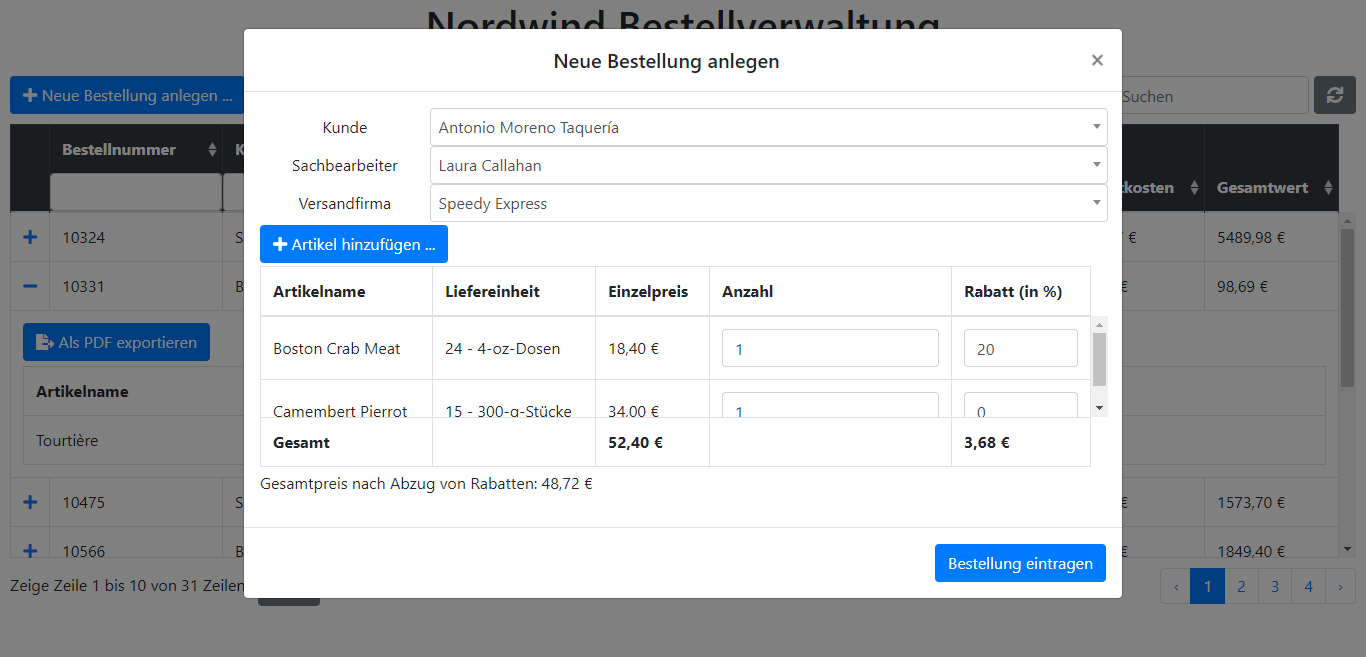
\includegraphics[scale=0.45]{Screenshots/CreateOrderDialog.png}}
            \caption{Bestellung anlegen Dialog}
        \end{figure}

        \newpage


    % 2.3
    \subsection{Funktionsweise}

    Die Anwendung besteht aus zwei Teilen, dem Server (backend) und dem Client (frontend) Teil.

    Der Server stellt Clients Möglichkeiten zur Verfügung, eine Webseite sowie Ergebnisse von vorgefertigten Datenbankabfragen abzurufen. Außerdem erlaubt er ihnen, Bestellungen anzulegen.

    Das Sortieren von Daten geschieht clientseitig, um eine unnötige Belastung der Datenbank zu vermeiden.

    Die Seite ist eine Single Page Application, das heißt, sie wird einmal geladen und danach nicht mehr automatisch neu geladen. Stattdessen werden Daten vom Server bei Bedarf nachgeladen und mithilfe von JavaScript in die aktuelle Seite eingefügt.


    % 2.4
    \subsection{Verwendete Technologien}
    Zur Realisierung des Projekts wurde mit folgenden Technologien gearbeitet:

    \begin{itemize}
        \item Node.js (Webserver, backend) %todo: Link
        \item HTML/CSS/JavaScript (Webseite, frontend)
        \item MySQL (Datenbank) %todo: Link
    \end{itemize}

    \newpage

    % 2.5
    \subsection{Verwendete Bibliotheken und Module}

        \subsubsection{backend}

            \paragraph{body-parser}
            Wird von express benötigt, um JSON Objekte mit POST Anfragen empfangen und verarbeiten zu können

            \paragraph{express}
            Erlaubt eine einfache Definition von Routen und eine Zuordnung von entsprechenden Serverantworten.

            \paragraph{mysql}
            Erlaubt den Zugriff auf MySQL Datenbanken

            \paragraph{nunjucks}
            Template Engine, mit dem man leicht verständliche Text templates erstellen kann.\\
            In diesem Projekt wird das Modul verwendet um die HTML Seite in wiederverwendbare, leichter wartbare Teile aufzuteilen.
            Außerdem werden damit Datenbankabfragen mit variablen Inhalten realisiert (wie etwa die Bestelldetails Abfrage).

            \newpage


        \subsubsection{frontend}

            \paragraph{@fortawesome/fontawesome-free}
            Stellt Symbole bereit, die mit \lstinline{<i class="fa far-<icon name>">} in die Seite eingebunden werden können.\\
            "`fa"' steht für fontawesome, diese Klasse muss in jedem icon Element vorhanden sein da sie grundlegende Dinge wie z.B. Höhe und Breite des Symbols definiert.\\
            "`far"' steht für "`fontawesome regular"', d.h. die Icons sind mit "`normalen"' Linien gezeichnet und große Teile des Icons sind durchsichtig.\\
            "`fas"' steht für "`fontawesome solid"', d.h. große Flächen der Icons sind farbig gefüllt womit diese gut sichtbar sind.\\
            Die Farbe der Icons kann dabei mit CSS festgelegt werden, indem man das icon Element selektiert und ihm eine ``color'' zuweist.

            \paragraph{bootstrap}
            Framework, das vorgefertigte CSS Klassen und JavaScript Funktionen bereit stellt (z.B. Dialoge). Damit kann man relativ schnell gut aussehende Webseiten erstellen.

            \paragraph{bootstrap-table}
            Framework zum Erstellen von Ausgabetabellen. Stellt auch nützliche Dinge wie Aufteilen in Seiten, Filter, Sortieren, usw. zur Verfügung.\\
            Dieses Modul wird für sämtliche Ausgabetabellen in der Anwendung verwendet.

            \paragraph{deep-eql}
            Kann Objekte auf Gleichheit überprüfen, ohne dass es sich um diesselbe Instanz handeln muss (unabhängig von der Reihenfolge der Attribute)

            \paragraph{flatpickr}
            Stellt Eingabe-Möglichkeiten für ein einzelnes Datum oder einen Datumsbereich zur Verfügung

            \paragraph{jquery}
            Vereinfacht das Finden und Manipulieren von Elementen im DOM, bietet auch nützliche Funktionen und Events wie z.B. Warten, bis das gesamte Dokument geladen ist

            \paragraph{jquery-ui}
            Bietet zahlreiche Effekte, Widgets, usw. Wird hier verwendet, um z.B. Dialoge verschiebbar zu machen

            \paragraph{jspdf}
            Ermöglicht es, im Browser PDF Dateien zu generieren

            \paragraph{jspdf-autotable}
            jspdf Erweiterung, die das einfache Einfügen von Tabellen in ein jspdf PDF Dokument erlaubt

            \paragraph{native-toast}
            Erlaubt es, Pop-Up Nachrichten anzeigen zu lassen, die nach kurzer Zeit wieder verschwinden (Heißt Toast weil es wie ein Toast von unten nach oben fliegt)

            \paragraph{popper.js}
            Ermöglicht das Darstellen von Sprechblasen, ist eine Abhängigkeit von bootstrap-table

            \paragraph{select2}
            Verbesserte Combobox, die zahlreiche Zusatzfunktionen wie etwa eine Suchfunktion zur Verfügung stellt

            \newpage


% 3.
\section{Funktionen der einzelnen Dateien}

    \subsection{/}
    Das Hauptverzeichnis beinhaltet die package.json und die Einstiegsdatei der Anwendung.

    \subsubsection{package.json}
    Beinhaltet Informationen über das Projekt, Skripte (die mit ``npm run <name>'' ausgeführt werden können) und Bibliotheken, die das Projekt benötigt.\\
    Die Bibliotheken wurden mit dem Paketmanager "`npm"' installiert, welcher für die Verwaltung der node module zuständig ist.\\
    Mit ``npm install <paket name> -{}-save'' kann man neue Module installieren und in der package.json speichern lassen. Module könne auf \href{https://www.npmjs.com/}{npmjs.com} gesucht werden.\\
    Andere Entwickler können im selben Verzeichnis wie die package.json den Befehl ``npm install'' ausführen, um sämtliche aufgelistete Module in der höchsten kompatiblen Version zu installieren.
    Die Module werden in dem Ordner ``node\_modules'' im Projekt gespeichert.

    \subsubsection{package-lock.json}
    Beinhaltet die tatsächlich installierten Module. Das sind nicht nur die in package.json aufgelisteten sondern auch deren Abhängigkeiten.\\
    Damit lässt sich die Version der einzelnen Module fixieren, damit jeder Entwickler exakt die gleichen Versionen installiert.


    \subsubsection{main.js}
    Die Einstiegsdatei, die in der package.json als ``main'' definiert wurde.\\
    Hier wird eine Verbindung zur Datenbank aufgebaut mithilfe des "`mysql"' Moduls und es wird eine WebServer Instanz erstellt und initialisiert.

    \subsubsection{.gitignore}
    Da das Projekt in einem git repository liegt gibt es auch eine .gitignore Datei, die Muster in Dateipfaden definiert, die von git ignoriert werden sollen. In diesem Fall ist das der gesamte node\_modules Ordner.


    \newpage


    \subsection{/src/backend}

    Beinhaltet den Quellcode der serverseitig genutzt wird.

        \subsubsection{SelectQueryExecutor}
        Stellt alle SQL Abfragen bereit, die ein Nutzer auslösen kann.\\
        Die Abfragen werden mit dem "`nunjucks"' template engine gerendert, damit Werte dynamisch eingesetzt werden können (wie z.B. die BestellNr bei der BestellDetails Abfrage).

        \subsubsection{WebServer}
        Sorgt dafür, dass Nutzer die Webseite nutzen können. Dazu nutzt er das "`express"' Modul, mit dem Routen definiert werden können auf die die Nutzer Zugriff haben. Diese können dann über "`localhost:8080/<route name>"' aufgerufen werden.

        Die zur Verfügung gestellten Routen sind:

        \begin{enumerate}
            \item Die HTML Seiten (hier nur index via "`localhost:8080/"')
            \item Externe Bibliotheken für das frontend (wie z.B. jQuery, bootstrap, etc.)
            \item Eigene JavaScript und CSS Dateien für das frontend
            \item Die nutzbaren Datenbankabfragen
        \end{enumerate}

        \subsubsection{OrderCreator}
        Ermöglicht es, Bestellungen anhand von Objekten in der Datenbank einzutragen.

        \paragraph{OrderCreator}
        Überträgt die Daten aus einem vom Nutzer überlieferten ``order'' Objekt in die Datenbank.
        Dazu wird zuerst das Objekt auf Richtigkeit überprüft, danach wird eine "`Transaction"' gestartet. Dann werden die benötigten SQL Befehle an das Datenbankmanagementsystem übertragen und schließlich mit "`commit"' ausgeführt.
        Der Vorteil von einer Transaction ist, dass bei Auftreten eines Fehlers keine Teildaten in der Datenbank stehen, sondern entweder alles oder nichts. Außerdem ist eine solche Abfrage schneller, weil die SQL Befehle vom DBMS erst gesammelt und dann alle auf einmal geparst werden.

        \paragraph{OrderValidator}
        Überprüft ein ``order'' Objekt auf Richtigkeit. Hier wird zum einen die Struktur des Objekts geprüft (sind alle Felder vorhanden und haben den richtigen Variablentyp?) und zum anderen die Inhalte validiert (gibt es diesen Kunden, Lieferanten, Artikel?, Ist der Rabatt zwischen 0 und 100\%?).
        Diese Klasse wird vom OrderCreator verwendet, um das ``order'' Objekt zu validieren.


        \newpage


        \subsection{/src/frontend}
        Beinhaltet den Quellcode der clientseitig genutzt wird.

        Das frontend ist unterteilt in drei Bereiche:

        \begin{itemize}
            \item css: Beinhaltet Cascading Stylesheets (zuständig für das Aussehen der Webseite, z.B. Farben, Positionierung, Größe von Elementen, usw.)
            \item javascript: Beinhaltet JavaScript Dateien (zuständig für das Verhalten der Webseite, z.B. "`Öffne einen Dialog wenn auf diesen Knopf geklickt wird"', "`Sende eine Anfrage an den Server bei Absenden dieses Formulars"')
            \item templates: Beinhaltet die HTML Templates (definieren die Struktur der Seiten, d.h. welche Elemente gibt es und wie sind sie ineinander verschachtelt)
        \end{itemize}

        Jeder dieser Bereiche ist nochmals unterteilt in Seiten spezifische Dateien (hier nur index) und Dateien, die für alle Seiten genutzt werden können (util).


        \newpage


        \subsubsection{templates}
        Die Template Dateien sind "`nunjucks"' Templates. Diese werden vom WebServer gerendert und dann an den Nutzer übertragen.
        Die Dateiendung "`njk"' soll nur darauf hinweisen, dass es nunjucks Templates sind, es könnte aber jede beliebige Endung sein.
        Das Basisverzeichnis für Templates wird im WebServer konfiguriert.

        Die Vorteile vom Nutzen solcher Templates sind:

        \begin{enumerate}
            \item Teile können wiederverwendbar gemacht werden, z.B. das Dialog Basis Template
            \item HTML Dateien können in übersichtliche Dateien aufgeteilt werden (hier sind z.B. index, external libraries, internal libraries und dialogs voneinander getrennt, obwohl diese im gerenderten Template alle vereint sind)
            \item Kommentare in den Templates werden nicht mit übertragen (so wie es bei HTML Kommentaren der Fall wäre)
        \end{enumerate}



            \paragraph{util}
            Beinhaltet Templates die auf jeder Seite verwendet werden können.

                \subparagraph{dialog.njk}
                Basis Template für Dialog Container. Dies ist größtenteils vom Beispiel von bootstrap übernommen worden. Hier wurden Variablen genutzt (\lstinline|{{ variablenName }}|), um Texte einzusetzen, wie Dialog Element ID und Titel.
                Außerdem wurden Blöcke verwendet (\lstinline||), die komplett ersetzt werden können durch von child templates definierte Blöcke.

            \paragraph{index}
            Beinhaltet alle Templates die auf der index Seite zum Einsatz kommen.

                \subparagraph{dialogs}
                Hier werden die benötigten Dialog Container für die index Seite definiert (Artikel hinzufügen, Bestellung anlegen und Lagerbestandswarnungen). Diese Dateien sind alle gleich aufgebaut.\\
                Zuerst wird angegeben, dass das Template ableitet vom Basisdialog Template (\lstinline||), dann werden die Variablen gesetzt, die im Basisdialog benutzt werden (\lstinline||) und schließlich werden die Blöcke definiert, die der Basisdialog bereitstellt (auch mit \lstinline|| aber diesmal mit Inhalten zwischen den beiden tags).


                \subparagraph{libraries}
                Zur Übersichtlichkeit wurde das Einbinden der Bibliotheken und stylesheets in diese Dateien ausgelagert.\\
                Hier werden mit \lstinline{<script src="pfad-zum-skript"></script>} JavaScript Dateien\\ und mit \lstinline{<link rel="stylesheet" href="pfad-zur-css-datei">} stylesheet Dateien vom Server geladen.

                Die external libraries sind dabei diejenigen, die als node module installiert wurden und die "`internal"' libraries die selbst geschriebenen Dateien.


                \subparagraph{index.njk}
                Hier wird die Seite, wie sie der Nutzer erhalten soll aus den anderen Teil-Templates zusammengebaut. Dazu wurde ein Standard HTML Gerüst aufgebaut, das diesem Schema folgt:


                \begin{lstlisting}
<html>
    <head>
        <title>Seitentitel in Tab Liste</title>
        ...
    </head>
    <body>
        ...
    </body>
</html>
                \end{lstlisting}

                \begin{itemize}
                    \item <html>: Hauptknoten
                    \item <head>: Beinhaltet meta Daten, Seitentitel und einzubindende Bibliotheken
                    \item <body>: Eigentlicher Inhalt der Seite
                \end{itemize}

                HTML Tags bestehen meistens aus einem öffnenden und schließenden Tag, und sämtlicher Text dazwischen sind ``child nodes'' und ``inner texts''. HTML Tags können auch Attribute haben, diese stehen im öffnenden Tag zwischen dem Namen und ``>'', z.B. \lstinline{<div id="mein-container">}.\\
                Die baumartige Darstellung dieser Verschachtelung von HTML tags wird auch DOM genannt ("`Document Object Model"').

                Im body gibt es einen Überschriftsteil ("`<header>"') und einen Hauptteil ("`<main>"').
                Hier wird ein leeres Tabellenelement und eine Toolbar für die Tabelle angelegt, die dann später mit JavaScript genutzt werden, um eine Ausgabetabelle zu generieren.

                Einzufügende Templates werden mit \lstinline|| angegeben und beim rendern werden diese tags durch das jeweilige template ersetzt.


        \newpage


        \subsubsection{css}

        In den css Dateien kann man mithilfe von Selektoren Elemente auswählen, die von einer bestimmten Konfiguration betroffen sein sollen.
        Der Aufbau eines solchen Selektors ist:


        \begin{lstlisting}
<element>.<Klasse>#<ID>:<Pseudo Klasse>
        \end{lstlisting}

        \begin{itemize}
            \item Element: Name des HTML Elements, z.B. body, h1, p
            \item Klasse: Name einer Klasse die das Element haben muss, die Klasse steht dabei im Element im Attribut ``class'' und kann statisch im HTML vergeben oder mit JavaScript während der Laufzeit vergeben werden. Ein Element kann mehrere Klassen gleichzeitig haben, die Klassen Name im ``class'' Attribut sind dann mit Leerzeichen voneinander getrennt.
            \item ID: Die ID, die das Element haben muss, diese sollte eindeutig sein und steht im ``id'' Attribut eines Elements
            \item Pseudo Klasse: Das ist eine Klasse, die vom Browser abhängig vom Zustand des Elements vergeben wird, z.B. die "`hover"' Klasse bekommt ein Element, wenn sich der Mauszeiger über ihm befindet.
        \end{itemize}


        Ein Selektor muss mindestens Element Name, Klasse oder ID enthalten, valide Selektoren sind z.B. "`body"', "`.section-title"' und "`\#orders-table"'

        Der Aufbau einer CSS Konfiguration ist:

        \begin{lstlisting}
<Selektor> (, <Selektor>, ...) {
  Eigenschaft: Wert,
  Eigenschaft: Wert,
  ...
}
        \end{lstlisting}


        Mögliche Konfigurationswerte sind z.B. padding, text-align oder height.


        \newpage


        \subsubsection{javascript}

        Hier sind alle JavaScript Dateien gesammelt.
        Die meisten Dateien sind Klassen, die mithilfe von Prototypen erstellt wurden.\\

        Prototypen sind quasi dasselbe wie Klassen in JavaScript, der Konstruktor ist eine Funktion und die Klassenmethoden werden in der ``prototype'' Eigenschaft der Klasse definiert. Attribute werden nirgendswo deklariert sondern einfach in den Methoden mit \lstinline{this.<attribut name>} gesetzt oder ausgelesen.

        Vererbung geschieht, indem im Konstruktor der Child Klasse der Konstruktor der parent Klasse aufgerufen wird mit \lstinline{Elternklasse.call(this, <args)}.
        Das erste Argument ist dabei die Instanz der child Klasse(``this''), die an den Konstruktor der Elternklasse übergeben wird. Wann immer im Konstruktor der Elternklasse dann ``this'' benutzt wird, wird die Instanz der child Klasse genutzt.

        Danach muss der prototype der Klasse noch angepasst werden, indem zunächst mal der komplette prototype der Elternklasse kopiert wird. Das geschieht mit \lstinline{Object.create(Elternklasse.prototype)}.\\
        Zum Schluss muss die ``constructor'' Methode ersetzt werden durch den Konstruktor der child Klasse.\\
        Dann können weitere Methoden hinzugefügt oder vorhandene überschrieben werden, indem die Attribute des prototype Objekts mit den gewünschten Methoden gesetzt werden.\\
        Die parent Methoden können aufgerufen werden, indem sie aus der parent Klasse abgerufen werden (\lstinline{Elternklasse.<methode>}) und dann mit ``.call()'' aufgerufen werden und als ``this'' die Instanz des child Objekts übergeben wird (analog des Aufrufs im Konstruktor).


        \paragraph{util/DataFetcher}
        Lädt Daten vom Server mit ajax requests ("`Asynchronous JavaScript and XML"' ).
        Stellt außerdem Cache-Funktionalitäten bereit, damit die gleichen Daten nicht mehrmals innerhalb kurzer Zeit vom Server abgefragt werden müssen.

        \paragraph{util/Dialog}
        Basisklasse für Dialoge. Erstellt einen bootstrap Dialog aus einem Dialogcontainer und verwaltet das Dialog Element.

        \paragraph{util/Utils}
        Statische Funktionen, die überall verwendet werden können. Dazu zählen Zahlenformatierer (Euro, Prozent) und Statusmeldungen (Erfolgs- und Fehlermeldung)

        \paragraph{util/Table/Table}
        Eine Basisklasse für eine Tabelle. Benutzt bootstrap-table, ermöglicht aber das Verwenden von zusätzlichen benutzerdefinierten Filter, die nicht mit bootstrap-table erstellt werden können (in diesem Fall nur der Datumsbereich Filter).

        \paragraph{util/Table/Filter/Filter}
        Eine Basisklasse für Filter, basierend auf der select2-filter Erweiterung von bootstrap-table.

        \paragraph{util/Table/Filter/DateRangeFilter}
        Fügt einen Datumsbereichfilter zur Tabelle hinzu. Benutzt dazu flatpickr.


        \paragraph{index/Dialog/AddArticleDialog}
        Klasse für den Dialog, mit dem ein Artikel zur Bestellung hinzugefügt werden kann.

        \paragraph{index/Dialog/CreateOrderDialog}
        Klasse für den Dialog, mit dem eine neue Bestellung angelegt und gespeichert werden kann.
        Beinhaltet außerdem eine Ausgabetabelle, mit der die bisherigen Bestell-Artikel visualisiert werden und eine Order sowie OrderArticle Klasse, mit der die aktuelle Bestellung gespeichert und ans backend übertragen werden kann.

        \paragraph{index/Dialog/StocksWarningsDialog}
        Klasse für den Dialog, in dem Lagerbestandswarnungen angezeigt werden.

        \paragraph{index/OrdersTable}
        Beinhaltet die Klassen, die für das Anzeigen der Bestellübersichtstabelle zuständig sind.
        Darin ist auch die Tabelle für die Bestelldetails, die beim Aufklappen einer Bestellung dynamisch eingefügt wird.
        Außerdem ist hier auch eine Klasse, um Bestelldaten in eine PDF Datei umzuwandeln


    \newpage


% 4
\section{Noch zu erledigende Dinge}

Die vorliegende Anwendung ist nur eine erste Version, die aber die erforderten Funktionalitäten erfüllt. Natürlich ist noch nicht alles perfekt, zum Teil ist auch noch alter Code vorhanden der refactored werden müsste.

Die folgenden Dinge könnten in der Zukunft noch in Angriff genommen werden:

\begin{itemize}
    \item "`provider"' überall ersetzen durch "`shipper"'
    \item OrderValidator: Prüfen, dass keine Bestellartikel ID doppelt vorkommt
    \item "`setCustomValidity"' benutzen, um Fehler in Formularen hervorzuheben (in dem "`Neue Bestellung anlegen"' Dialog)
    \item Möglichkeit zum Löschen hinzugefügter Artikel in der Bestellmaske einbauen
    \item Höhe der "`Bestellungen"' Tabelle automatisch an die Höhe des Browser Fensters anpassen (mit minimaler Höhe)
    \item Nach Hinzufügen einer Bestellung die "`Bestellungen"' Tabelle aktualisieren
    \item Die Combo Box Filter in der "`Bestellungen"' Tabelle durch eine eigene Filter Implementation ersetzen
\end{itemize}

\end{document}
